% pyRAMBO -- library overview (feature-oriented)
% Build:  pdflatex pyRAMBO_overview.tex   (run twice for the outline)
% Figures in figures/ are real pyRAMBO output, see make_figures.py.

\documentclass[aspectratio=169,10pt]{beamer}

\usetheme{Madrid}
\usepackage[T1]{fontenc}
\usepackage{lmodern}
\usepackage{listings}
\usepackage{tikz}
\usetikzlibrary{arrows.meta, positioning, shapes.geometric, fit, backgrounds, calc, decorations.pathreplacing}

% ---------------------------------------------------------------- colours
\definecolor{ramboblue}{HTML}{1F5A99}
\definecolor{rambored}{HTML}{C0392B}
\definecolor{rambogreen}{HTML}{2E8B57}
\definecolor{rambogold}{HTML}{D68910}
\definecolor{rambogrey}{HTML}{ECEFF1}
\definecolor{rambopurple}{HTML}{7D3C98}

\setbeamercolor{palette primary}{bg=ramboblue,fg=white}
\setbeamercolor{palette secondary}{bg=ramboblue!85!black,fg=white}
\setbeamercolor{palette tertiary}{bg=ramboblue!70!black,fg=white}
\setbeamercolor{structure}{fg=ramboblue}
\setbeamercolor{title}{bg=ramboblue,fg=white}
\setbeamercolor{frametitle}{bg=ramboblue,fg=white}
\setbeamertemplate{navigation symbols}{}
\setbeamertemplate{blocks}[rounded][shadow=false]

% ---------------------------------------------------------------- code style
\lstdefinestyle{py}{
  language=Python,
  basicstyle=\ttfamily\footnotesize,
  keywordstyle=\color{ramboblue}\bfseries,
  commentstyle=\color{rambogreen}\itshape,
  stringstyle=\color{rambored},
  showstringspaces=false,
  backgroundcolor=\color{rambogrey},
  frame=none,
  xleftmargin=4pt, xrightmargin=4pt,
  aboveskip=2pt, belowskip=2pt,
  morekeywords={as},
}
\lstset{style=py}

% ---------------------------------------------------------------- tikz styles
\tikzset{
  node distance=7mm and 9mm,
  >={Stealth[length=2.6mm]},
  box/.style={rectangle, rounded corners=2pt, draw=ramboblue, fill=ramboblue!10,
              align=center, minimum height=7mm, inner sep=3pt, font=\footnotesize},
  boxr/.style={box, draw=rambored, fill=rambored!10},
  boxg/.style={box, draw=rambogreen, fill=rambogreen!10},
  boxo/.style={box, draw=rambogold, fill=rambogold!15},
  boxp/.style={box, draw=rambopurple, fill=rambopurple!10},
  boxk/.style={box, draw=black!60, fill=rambogrey},
  pkg/.style={box, minimum width=2.6cm, minimum height=9mm, font=\small\bfseries},
  flow/.style={->, thick, draw=black!70},
  flowb/.style={->, very thick, draw=ramboblue},
  flowr/.style={->, very thick, draw=rambored},
  flowd/.style={->, thick, dashed, draw=black!60},
  lbl/.style={font=\scriptsize, text=black!70},
}

\newcommand{\pr}{\textsc{pyRAMBO}}
\newcommand{\code}[1]{\texttt{#1}}

% ---------------------------------------------------------------- title
\title[pyRAMBO]{pyRAMBO}
\subtitle{A Bayesian-optimization toolbox for expensive simulations}
\author[Y.~Lecomte, M.~A.~Mendez]{Yannick Lecomte \and Miguel A.~Mendez}
\institute[VKI]{Machine Learning for Fluid Systems (ML4F)\\
  von Karman Institute for Fluid Dynamics}
\date{\today}

\begin{document}

\begin{frame}[plain]
  \titlepage
\end{frame}

% =============================================================== 1
\begin{frame}{What is \pr{}?}
  \begin{columns}[T]
    \column{0.52\textwidth}
    \textbf{R}ank-one \textbf{A}ccelerated \textbf{M}ulti-objective / fidelity / output
    for \textbf{B}ayesian \textbf{O}ptimization.
    \medskip

    \begin{itemize}
      \item Gaussian-process (GP) based \textbf{Bayesian optimization} (BO) for
            \emph{expensive black-box} objectives: CFD runs, experiments, training jobs.
      \item \textbf{Lightweight}: only \code{numpy}, \code{scipy}, \code{matplotlib}.
      \item \textbf{Three flavours}, one common look and feel.
      \item \textbf{Everything is a config object}: no hidden global state.
      \item Runs are \textbf{saved, logged and replayable}.
    \end{itemize}

    \column{0.46\textwidth}
    \begin{center}
    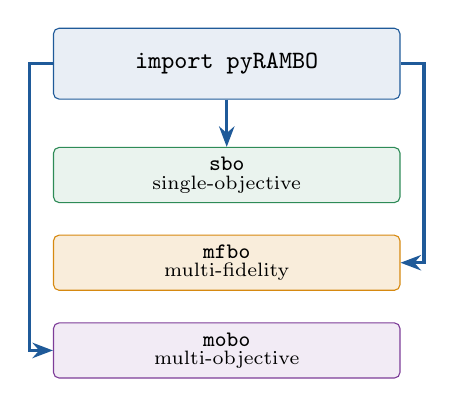
\begin{tikzpicture}
      \node[pkg, boxg, minimum width=4.4cm] (s) {\code{sbo}\\[-1mm]\scriptsize single-objective};
      \node[pkg, boxo, minimum width=4.4cm, below=4mm of s] (f) {\code{mfbo}\\[-1mm]\scriptsize multi-fidelity};
      \node[pkg, boxp, minimum width=4.4cm, below=4mm of f] (m) {\code{mobo}\\[-1mm]\scriptsize multi-objective};
      \node[pkg, minimum width=4.4cm, above=6mm of s] (p) {\code{import pyRAMBO}};
      \draw[flowb] (p) -- (s);
      \draw[flowb] (p.east) -- ++(3mm,0) |- (f.east);
      \draw[flowb] (p.west) -- ++(-3mm,0) |- (m.west);
    \end{tikzpicture}
    \end{center}
  \end{columns}
\end{frame}

% =============================================================== 2
\begin{frame}{The idea in one picture: the BO loop}
  \centering
  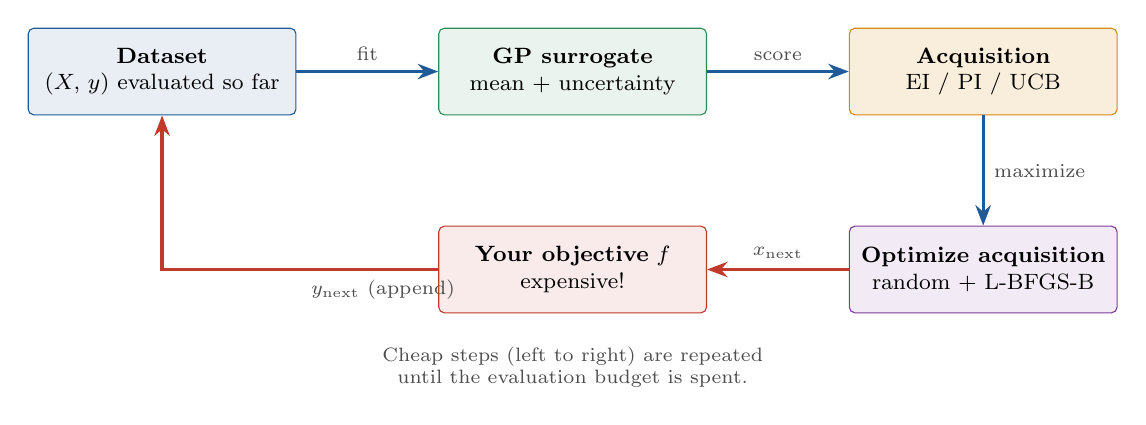
\begin{tikzpicture}[node distance=14mm and 18mm]
    \node[box, minimum width=3.4cm, minimum height=1.1cm] (data) {\textbf{Dataset}\\ $(X,\,y)$ evaluated so far};
    \node[boxg, minimum width=3.4cm, minimum height=1.1cm, right=of data] (gp) {\textbf{GP surrogate}\\ mean $+$ uncertainty};
    \node[boxo, minimum width=3.4cm, minimum height=1.1cm, right=of gp] (acq) {\textbf{Acquisition}\\ EI / PI / UCB};
    \node[boxp, minimum width=3.4cm, minimum height=1.1cm, below=of acq] (opt) {\textbf{Optimize acquisition}\\ random + L-BFGS-B};
    \node[boxr, minimum width=3.4cm, minimum height=1.1cm, left=of opt] (f) {\textbf{Your objective} $f$\\ expensive!};
    \draw[flowb] (data) -- node[above, lbl]{fit} (gp);
    \draw[flowb] (gp) -- node[above, lbl]{score} (acq);
    \draw[flowb] (acq) -- node[right, lbl]{maximize} (opt);
    \draw[flowr] (opt) -- node[above, lbl]{$x_{\rm next}$} (f);
    \draw[flowr] (f) -| node[below right, lbl, pos=0.25]{$y_{\rm next}$ (append)} (data);
    \node[lbl, below=3mm of f, text width=8cm, align=center] {Cheap steps (left to right) are repeated until the evaluation budget is spent.};
  \end{tikzpicture}

  \medskip
  \textbf{\pr{} implements every box of this loop}, so the only thing you provide is $f$ and the bounds.
\end{frame}

% =============================================================== 3
\begin{frame}{Library architecture}
  \centering
  \resizebox{!}{0.80\textheight}{%
  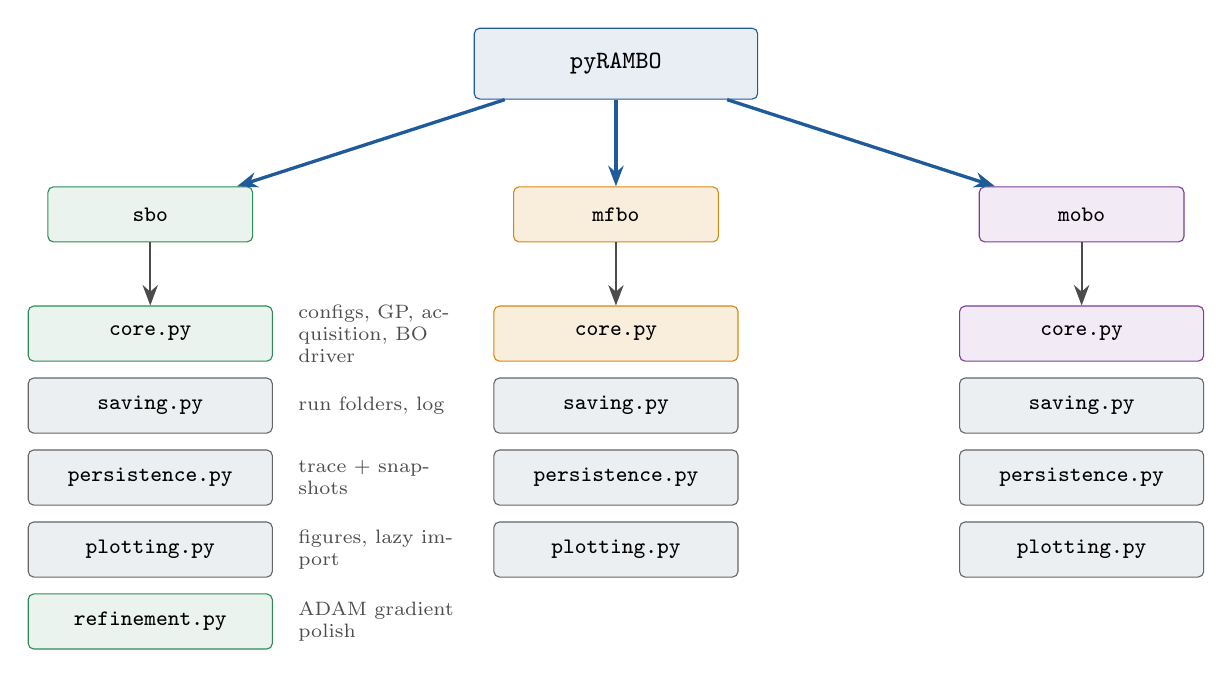
\begin{tikzpicture}[node distance=6mm and 5mm]
    % top
    \node[pkg, minimum width=3.6cm] (root) {\code{pyRAMBO}};
    % three packages
    \node[pkg, boxg, below left=11mm and 28mm of root] (sbo) {\code{sbo}};
    \node[pkg, boxo, below=11mm of root] (mfbo) {\code{mfbo}};
    \node[pkg, boxp, below right=11mm and 28mm of root] (mobo) {\code{mobo}};
    \draw[flowb] (root) -- (sbo);
    \draw[flowb] (root) -- (mfbo);
    \draw[flowb] (root) -- (mobo);

    % modules below each
    \foreach \p/\c in {sbo/boxg, mfbo/boxo, mobo/boxp}{
      \node[\c, minimum width=3.1cm, below=8mm of \p] (\p core) {\code{core.py}};
      \node[boxk, minimum width=3.1cm, below=2mm of \p core] (\p sav) {\code{saving.py}};
      \node[boxk, minimum width=3.1cm, below=2mm of \p sav] (\p per) {\code{persistence.py}};
      \node[boxk, minimum width=3.1cm, below=2mm of \p per] (\p plt) {\code{plotting.py}};
      \draw[flow] (\p) -- (\p core);
    }
    % extra module only in sbo
    \node[boxg, minimum width=3.1cm, below=2mm of sboplt] (sbor) {\code{refinement.py}};

    % descriptions
    \node[lbl, right=2mm of sbocore, text width=2.2cm] {configs, GP, acquisition, BO driver};
    \node[lbl, right=2mm of sbosav, text width=2.2cm] {run folders, log};
    \node[lbl, right=2mm of sboper, text width=2.2cm] {trace + snapshots};
    \node[lbl, right=2mm of sboplt, text width=2.2cm] {figures, lazy import};
    \node[lbl, right=2mm of sbor, text width=2.2cm] {ADAM gradient polish};
  \end{tikzpicture}}

  \vspace{-1mm}
  {\footnotesize Same four modules in every subpackage; the three are \textbf{independent} (no shared base, no cross imports).}
\end{frame}

% =============================================================== 4
\begin{frame}{Anatomy of a run: configs in, result out}
  \centering
  \resizebox{!}{0.82\textheight}{%
  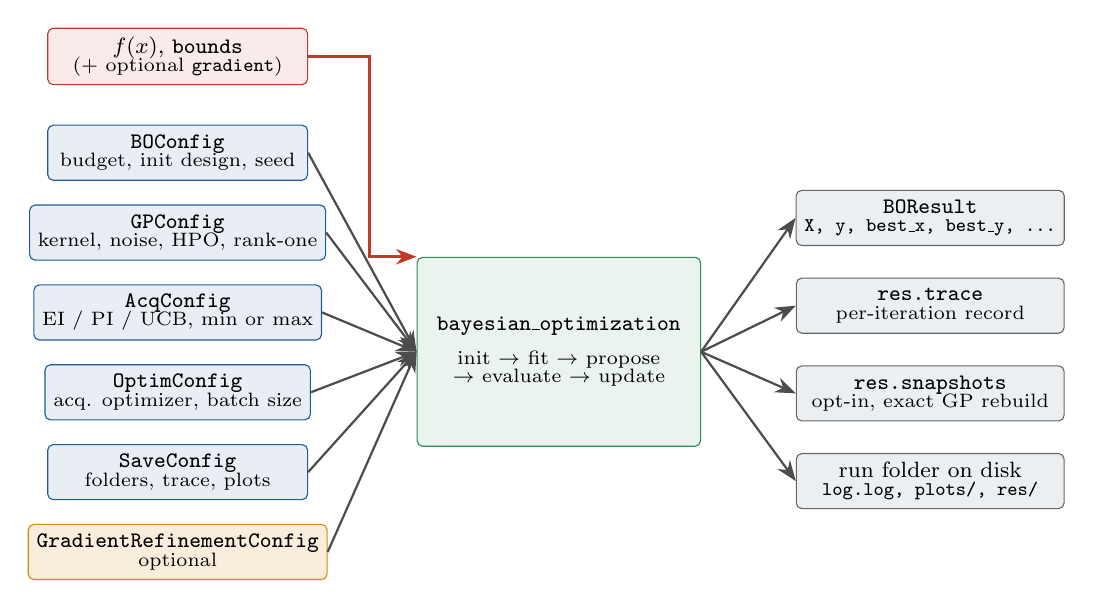
\begin{tikzpicture}[node distance=3mm and 14mm]
    % configs column
    \node[box, minimum width=3.3cm] (c1) {\code{BOConfig}\\[-1mm]\scriptsize budget, init design, seed};
    \node[box, minimum width=3.3cm, below=of c1] (c2) {\code{GPConfig}\\[-1mm]\scriptsize kernel, noise, HPO, rank-one};
    \node[box, minimum width=3.3cm, below=of c2] (c3) {\code{AcqConfig}\\[-1mm]\scriptsize EI / PI / UCB, min or max};
    \node[box, minimum width=3.3cm, below=of c3] (c4) {\code{OptimConfig}\\[-1mm]\scriptsize acq. optimizer, batch size};
    \node[box, minimum width=3.3cm, below=of c4] (c5) {\code{SaveConfig}\\[-1mm]\scriptsize folders, trace, plots};
    \node[boxo, minimum width=3.3cm, below=of c5] (c6) {\code{GradientRefinementConfig}\\[-1mm]\scriptsize optional};

    \node[boxr, above=5mm of c1, minimum width=3.3cm] (fobj) {$f(x)$, \code{bounds}\\[-1mm]\scriptsize (+ optional \code{gradient})};

    % driver
    \node[pkg, boxg, minimum width=3.6cm, minimum height=2.4cm, right=12mm of c3, yshift=-5mm] (drv)
      {\code{bayesian\_optimization}\\[1mm]\scriptsize init $\to$ fit $\to$ propose\\[-1mm]\scriptsize $\to$ evaluate $\to$ update};

    \foreach \c in {c1,c2,c3,c4,c5,c6}{ \draw[flow] (\c.east) -- (drv.west); }
    \draw[flowr] (fobj.east) -| ([xshift=-6mm]drv.north west) -- (drv.north west);

    % outputs
    \node[boxk, minimum width=3.4cm, right=12mm of drv, yshift=17mm] (res)
      {\code{BOResult}\\[-1mm]\scriptsize \code{X, y, best\_x, best\_y, \dots}};
    \node[boxk, minimum width=3.4cm, below=4mm of res] (trace) {\code{res.trace}\\[-1mm]\scriptsize per-iteration record};
    \node[boxk, minimum width=3.4cm, below=4mm of trace] (snap) {\code{res.snapshots}\\[-1mm]\scriptsize opt-in, exact GP rebuild};
    \node[boxk, minimum width=3.4cm, below=4mm of snap] (disk) {run folder on disk\\[-1mm]\scriptsize \code{log.log, plots/, res/}};
    \foreach \o in {res,trace,snap,disk}{ \draw[flow] (drv.east) -- (\o.west); }
  \end{tikzpicture}}
\end{frame}

% =============================================================== 5
\begin{frame}[fragile]{Quickstart: a complete run in a few lines}
\begin{lstlisting}
from pyRAMBO import sbo as bo

f = lambda x: (x[0] - 0.7) ** 2   # objective to minimize

res = bo.bayesian_optimization(
    f=f,
    bounds=[(-2.0, 2.0)],
    bo_cfg=bo.BOConfig(n_init=5, n_iter=15, random_state=0),
    gp_cfg=bo.GPConfig(),
    acq_cfg=bo.AcqConfig(),
    optim_cfg=bo.OptimConfig(),
    save_cfg=bo.SaveConfig(),
)
print(res.best_x, res.best_y)
\end{lstlisting}
  \begin{columns}[T]
    \column{0.5\textwidth}
    \begin{block}{Same pattern for the other flavours}
      \footnotesize
      \code{from pyRAMBO import mfbo}\\
      \code{mfbo.multi\_fidelity\_bayesian\_optimization}\\[1mm]
      \code{from pyRAMBO import mobo}\\
      \code{mobo.multi\_objective\_bayesian\_optimization}
    \end{block}
    \column{0.46\textwidth}
    \begin{block}{Install}
      \footnotesize
      \code{pip install -e ".[test]"}\\
      Python $\ge 3.9$.
    \end{block}
  \end{columns}
\end{frame}

% =============================================================== 6
\begin{frame}{Features at a glance}
  \small
  \begin{tabular}{@{}p{0.31\textwidth}p{0.64\textwidth}@{}}
    \hline
    \textbf{Feature} & \textbf{What you get}\\
    \hline
    Acquisition functions & Expected Improvement, Probability of Improvement, Upper Confidence Bound; min or max via one flag\\
    Hyperparameter learning & marginal-likelihood maximization (L-BFGS-B), every $k$ iterations, with safe default bounds\\
    Rank-one Cholesky update & extend the GP factor with new points instead of refactorizing\\
    Initial design & Latin hypercube or uniform; or bring your own \code{X\_init, y\_init}\\
    Acquisition optimizers & random, grid, or global search $+$ local L-BFGS-B refinement\\
    Diverse batch proposals & several well-separated candidates per iteration\\
    Gradient refinement & polish each proposal with projected ADAM if you have adjoint/AD gradients\\
    Multi-fidelity & cheap and expensive model combined, cost-aware (\code{mfbo})\\
    Multi-objective & Pareto front via expected hypervolume improvement (\code{mobo})\\
    Persistence \& replay & per-iteration trace; opt-in snapshots to rebuild any past posterior\\
    Built-in plots & state, convergence, history; GIF-ready frames\\
    \hline
  \end{tabular}
\end{frame}

% =============================================================== 7
\begin{frame}{Seeing the loop work: 1D noisy objective (\code{sbo})}
  \centering
  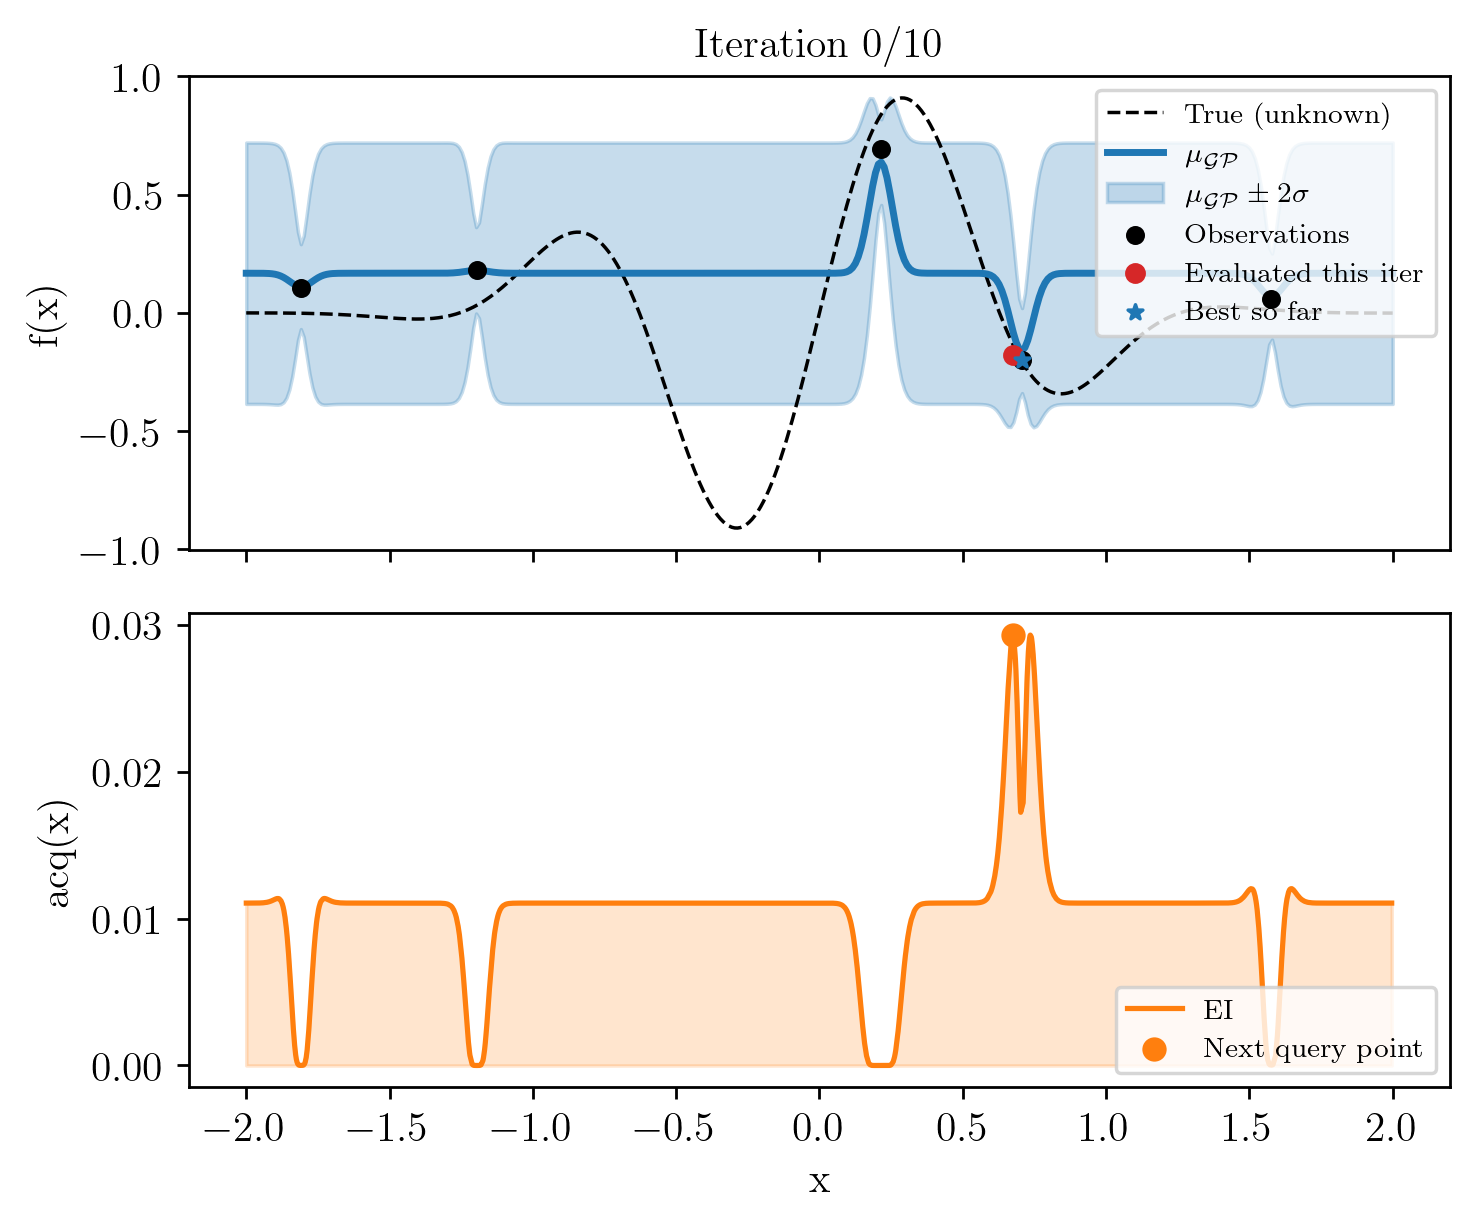
\includegraphics[width=0.325\textwidth]{figures/sbo1d_it00.png}\hfill
  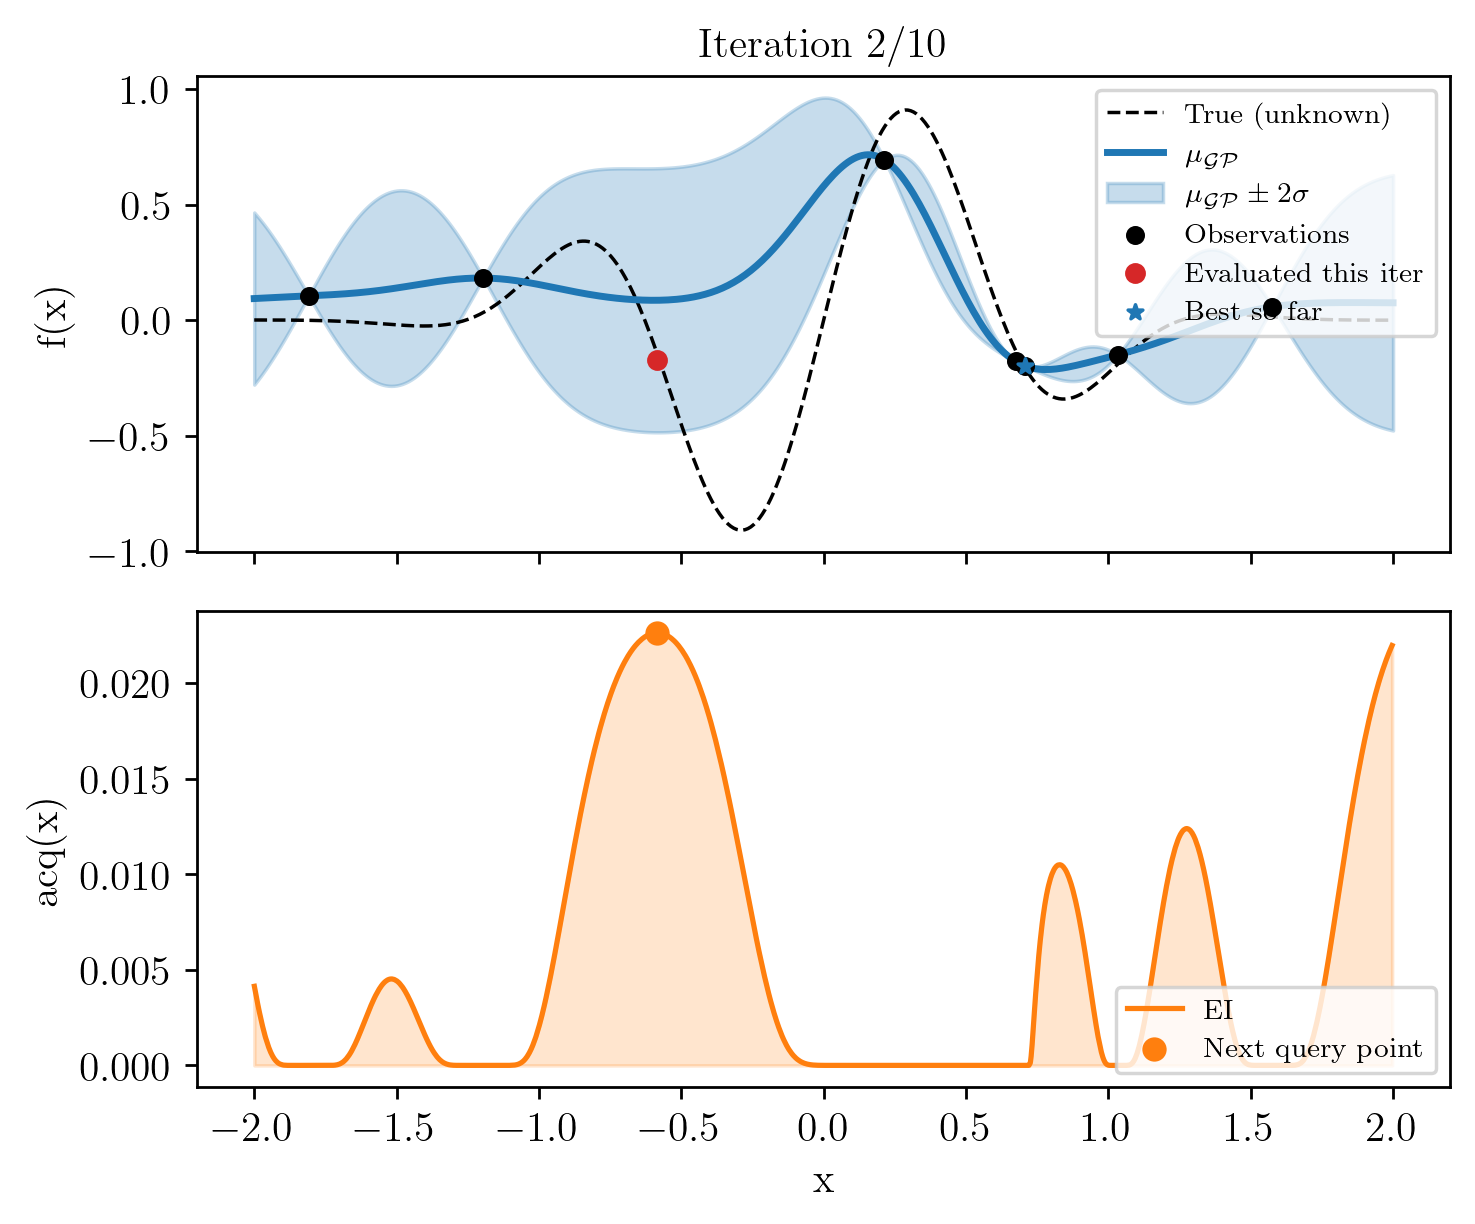
\includegraphics[width=0.325\textwidth]{figures/sbo1d_it02.png}\hfill
  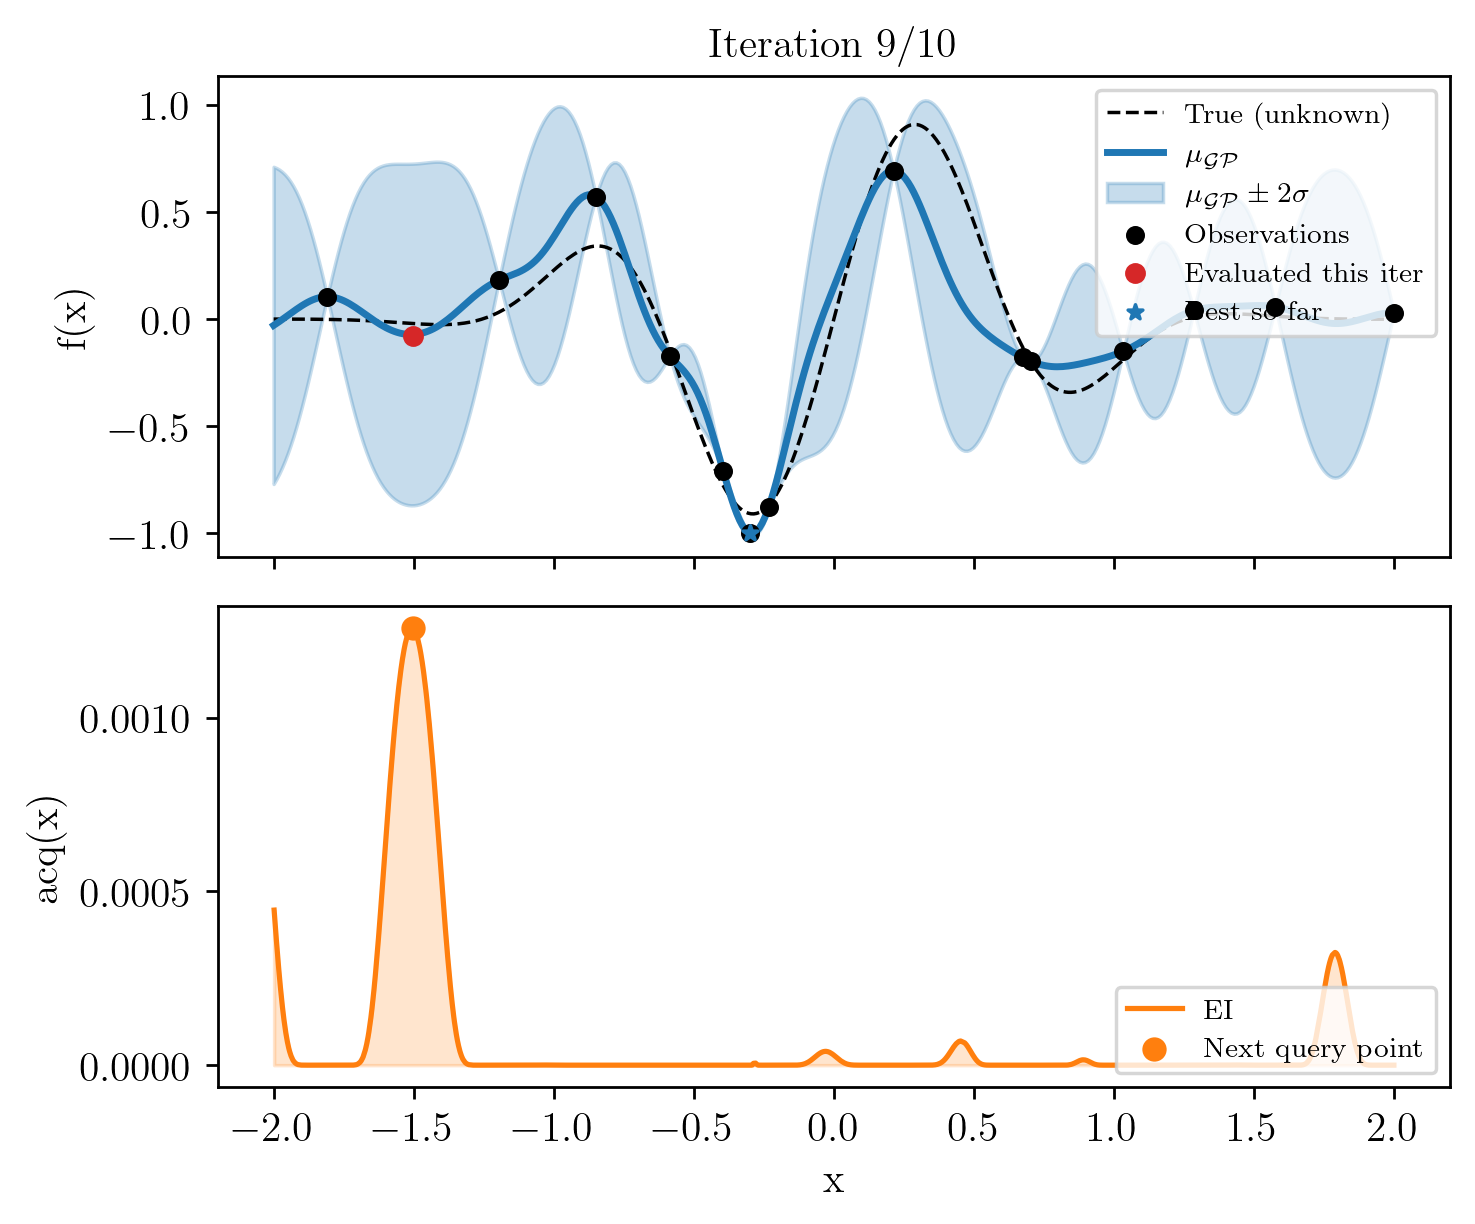
\includegraphics[width=0.325\textwidth]{figures/sbo1d_it09.png}

  \medskip
  \begin{columns}[T]
    \column{0.31\textwidth}\footnotesize \textbf{Top:} GP mean, $\pm 2\sigma$ band, observations, best so far.\\
    \textbf{Bottom:} acquisition and the chosen next point.
    \column{0.31\textwidth}\footnotesize The uncertainty collapses where we sample; EI trades off exploiting the best region against exploring wide-band regions.
    \column{0.31\textwidth}\footnotesize Produced by the library itself: \code{SaveConfig(plt\_all=True)}.
  \end{columns}
\end{frame}

% =============================================================== 9
\begin{frame}{Feature: rank-one Cholesky update}
  \begin{columns}[T]
    \column{0.5\textwidth}
    \textbf{Problem.} Every iteration adds a point; the GP needs the Cholesky factor of the kernel matrix. Refactorizing from scratch costs $\mathcal{O}(n^3)$.

    \medskip
    \textbf{\pr{}.} Keep the factor and \emph{append} the new rows: $\mathcal{O}(n^2)$ per new point. Works for several new points at once (batch, refinement).

    \medskip
    \begin{block}{When is it used?}
      \footnotesize
      \code{GPConfig(rank\_one=True, rank\_one\_threshold=1000)}\\
      Only in iterations \emph{without} a hyperparameter refit, and once the data set exceeds the threshold. A test checks it equals a full refit.
    \end{block}

    \column{0.48\textwidth}
    \centering
    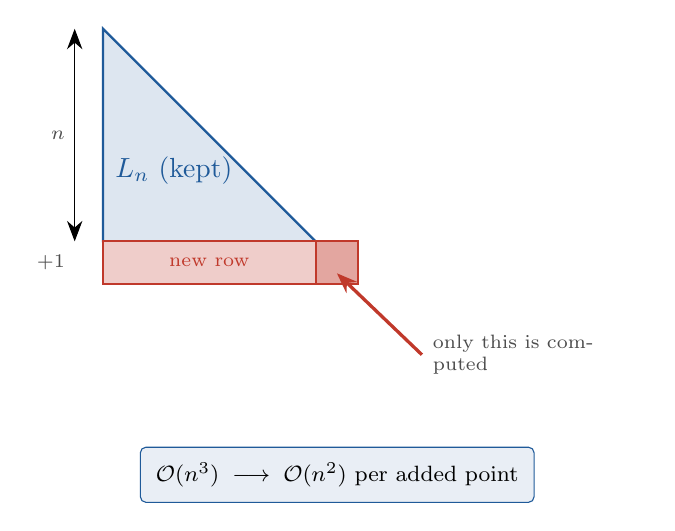
\begin{tikzpicture}[scale=0.9]
      % old factor
      \fill[ramboblue!15] (0,0) -- (0,-3) -- (3,-3) -- cycle;
      \draw[ramboblue, thick] (0,0) -- (0,-3) -- (3,-3) -- cycle;
      \node[ramboblue] at (1,-2) {$L_n$ (kept)};
      % new row
      \fill[rambored!25] (0,-3) rectangle (3,-3.6);
      \draw[rambored, thick] (0,-3) rectangle (3,-3.6);
      \fill[rambored!45] (3,-3) rectangle (3.6,-3.6);
      \draw[rambored, thick] (3,-3) rectangle (3.6,-3.6);
      \node[rambored, font=\scriptsize] at (1.5,-3.3) {new row};
      \draw[flowr] (4.5,-4.6) node[right, lbl, text width=2.6cm]{only this is computed} -- (3.3,-3.45);
      % dimension arrows
      \draw[<->] (-0.4,0) -- node[left, lbl]{$n$} (-0.4,-3);
      \node[lbl, left] at (-0.4,-3.3) {$+1$};
      \node[box, below=8mm of current bounding box.south, minimum width=5cm] {$\mathcal{O}(n^3) \;\longrightarrow\; \mathcal{O}(n^2)$ per added point};
    \end{tikzpicture}
  \end{columns}
\end{frame}

% =============================================================== 10
\begin{frame}[fragile]{Feature: diverse batch proposals}
  \begin{columns}[T]
    \column{0.5\textwidth}
    Ask for several candidates per iteration, e.g.\ to launch parallel simulations:
\begin{lstlisting}
optim_cfg=bo.OptimConfig(
    n_candidates=4,
    batch_distance_scale=0.05,
)
\end{lstlisting}
    \begin{itemize}\footnotesize
      \item Candidates are picked \textbf{greedily}.
      \item Each pick \textbf{penalizes the acquisition near itself}, so the batch spreads out.
      \item \code{n\_candidates=1} is the classic loop.
    \end{itemize}

    \column{0.48\textwidth}
    \centering
    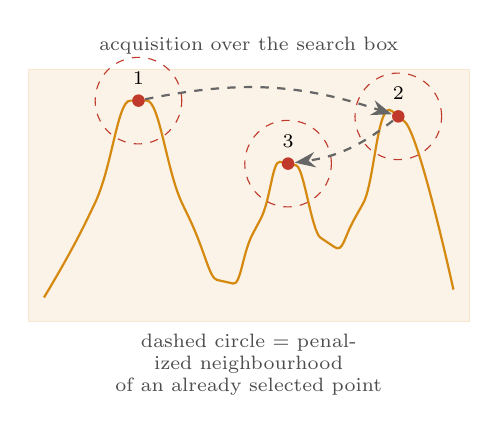
\begin{tikzpicture}[x=1cm,y=1cm]
      \draw[rambogold!20, fill=rambogold!10] (0,0) rectangle (5.6,3.2);
      \draw[rambogold, thick, rounded corners=3pt] plot[smooth, tension=0.8] coordinates {(0.2,0.3)(0.8,1.4)(1.4,2.8)(2.0,1.4)(2.5,0.5)(2.9,1.2)(3.3,2.0)(3.8,1.0)(4.2,1.4)(4.7,2.6)(5.4,0.4)};
      \node[lbl] at (2.8,3.5) {acquisition over the search box};
      \foreach \x/\y/\n in {1.4/2.8/1, 4.7/2.6/2, 3.3/2.0/3}{
        \node[circle, fill=rambored, inner sep=1.6pt, label={[font=\scriptsize]above:\n}] (p\n) at (\x,\y) {};
        \draw[rambored, dashed] (\x,\y) circle (0.55);
      }
      \draw[flowd] (p1) to[bend left=15] (p2);
      \draw[flowd] (p2) to[bend left=15] (p3);
      \node[lbl, text width=5cm, align=center] at (2.8,-0.55) {dashed circle = penalized neighbourhood\\ of an already selected point};
    \end{tikzpicture}
  \end{columns}
\end{frame}

% =============================================================== 11
\begin{frame}[fragile]{Feature: gradient refinement (adjoint / AD gradients)}
  \begin{columns}[T]
    \column{0.42\textwidth}
    If your solver gives $\nabla f$, let it finish the job:

    \smallskip
\begin{lstlisting}
res = bo.bayesian_optimization(
    f=f, gradient=grad_f, ...,
    refinement_cfg=
      bo.GradientRefinementConfig(
        enabled=True,
        n_steps=50,
        learning_rate=1e-2),
)
\end{lstlisting}
    \centering
    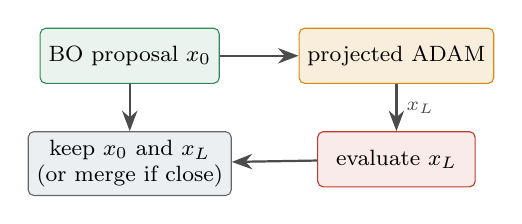
\begin{tikzpicture}
      \node[boxg, minimum width=2.0cm] (a) {BO proposal $x_0$};
      \node[boxo, minimum width=2.0cm, right=10mm of a] (b) {projected ADAM};
      \node[boxr, minimum width=2.0cm, below=6mm of b] (c) {evaluate $x_L$};
      \draw[flow] (a) -- (b);
      \draw[flow] (b) -- node[right, lbl]{$x_L$} (c);
      \node[boxk, minimum width=2.0cm, below=6mm of a] (d) {keep $x_0$ and $x_L$\\ (or merge if close)};
      \draw[flow] (a) -- (d);
      \draw[flow] (c) -- (d);
    \end{tikzpicture}

    \column{0.56\textwidth}
    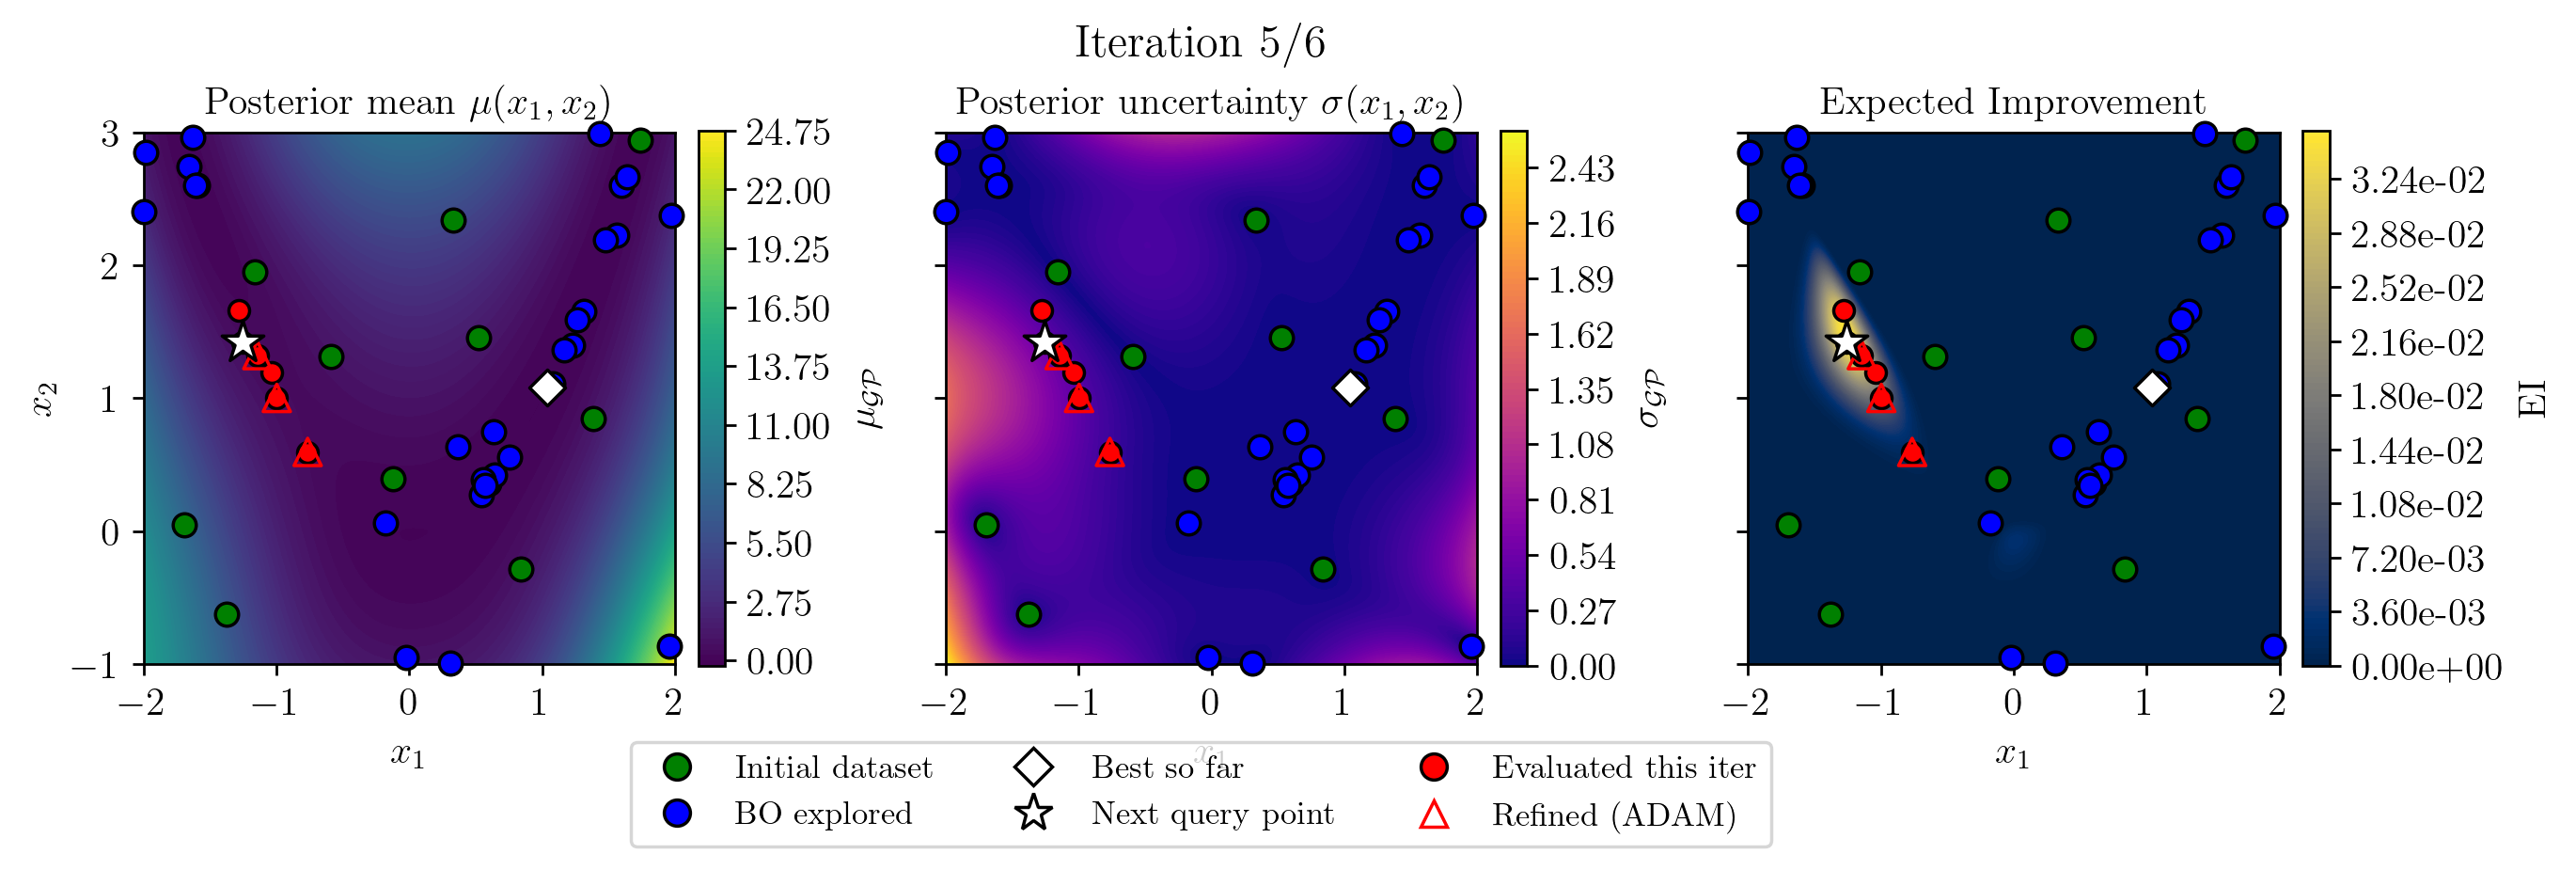
\includegraphics[width=\textwidth]{figures/refine_it05.png}

    {\scriptsize 2D state plot (Rosenbrock): posterior mean, uncertainty and EI. Red triangles: ADAM-refined endpoints; red dots: points evaluated this iteration. Global search by the GP, local polish by the gradient.}
  \end{columns}
\end{frame}

% =============================================================== 12
\begin{frame}{\code{mfbo}: multi-fidelity optimization}
  \begin{columns}[T]
    \column{0.47\textwidth}
    Combine a \textbf{cheap, biased} model with an \textbf{expensive, accurate} one.

    \smallskip
    \centering
    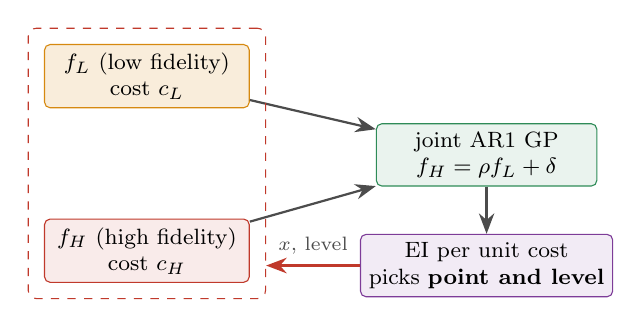
\begin{tikzpicture}[node distance=6mm and 10mm]
      \node[boxo, minimum width=2.6cm] (lo) {$f_L$ (low fidelity)\\ cost $c_L$};
      \node[boxr, minimum width=2.6cm, below=14mm of lo] (hi) {$f_H$ (high fidelity)\\ cost $c_H$};
      \node[boxg, minimum width=2.8cm, right=16mm of lo, yshift=-10mm] (gp) {joint AR1 GP\\ $f_H = \rho f_L + \delta$};
      \node[boxp, minimum width=2.8cm, below=6mm of gp] (acq) {EI per unit cost\\ picks \textbf{point and level}};
      \draw[flow] (lo) -- (gp);
      \draw[flow] (hi) -- (gp);
      \draw[flow] (gp) -- (acq);
      \node[draw=rambored, dashed, rounded corners=3pt, fit=(lo)(hi), inner sep=2mm] (grp) {};
      \draw[flowr] (acq.west) -- node[above, lbl]{$x$, level} (acq.west -| grp.east);
    \end{tikzpicture}

    \smallskip
    \raggedright\footnotesize
    \code{FidelityConfig(cost\_low=1, cost\_high=10)}.\\
    Two fidelity levels (Kennedy \& O'Hagan).

    \column{0.5\textwidth}
    \centering
    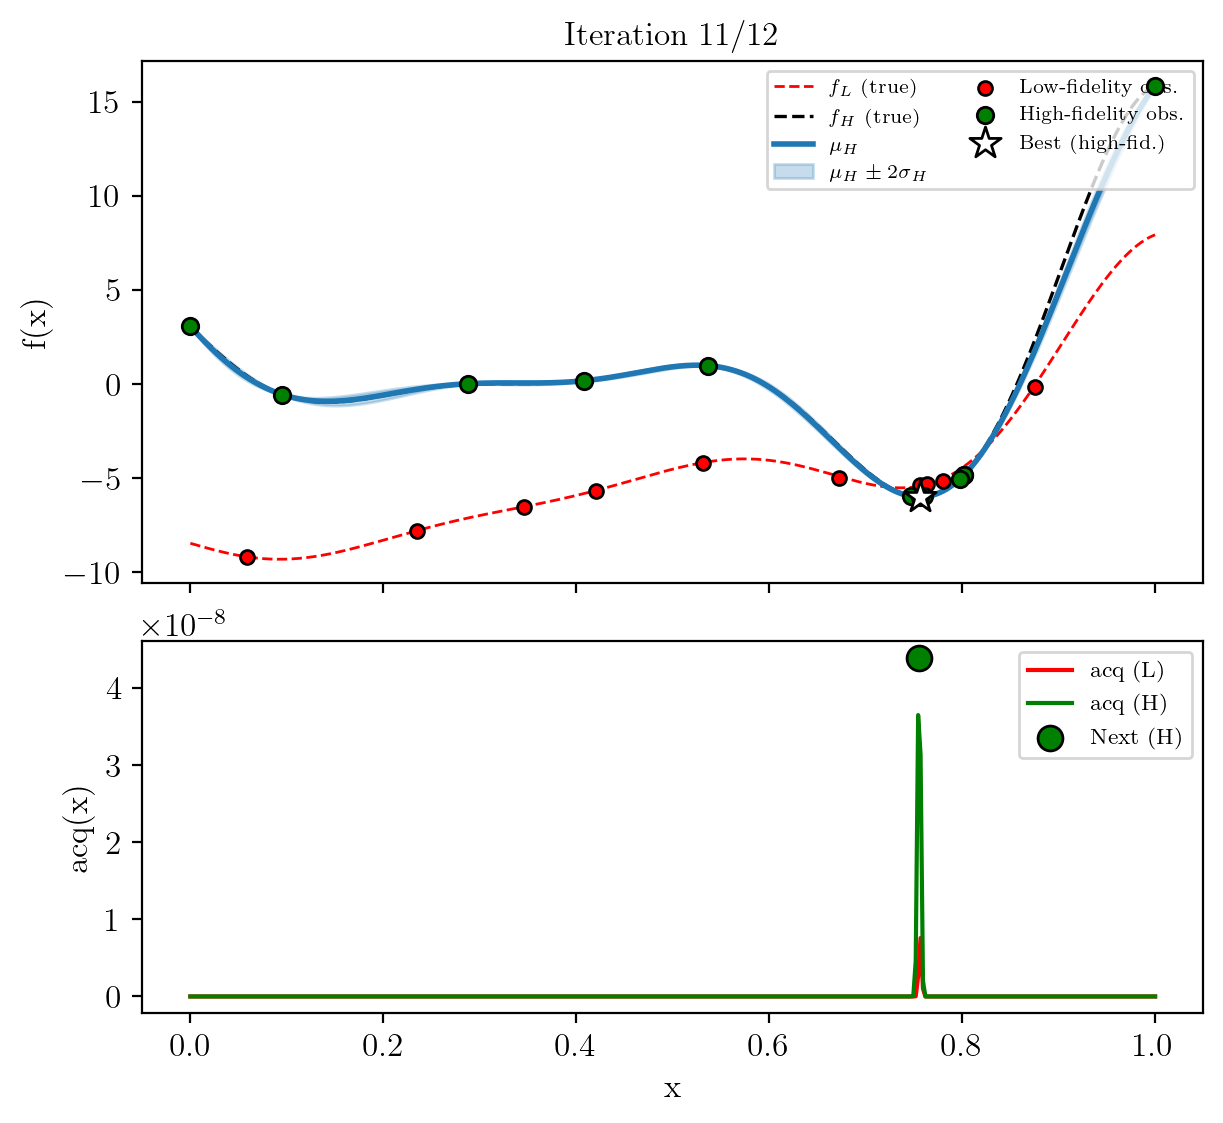
\includegraphics[height=0.66\textheight]{figures/mfbo_it11.png}

    {\scriptsize Forrester benchmark: red = cheap model and samples, green = expensive ones, $\mu_H$ = posterior of the expensive model.}
  \end{columns}
\end{frame}

% =============================================================== 13
\begin{frame}{\code{mobo}: multi-objective optimization}
  \begin{columns}[T]
    \column{0.52\textwidth}
    Several competing objectives $\Rightarrow$ a \textbf{Pareto front} instead of one optimum.

    \smallskip
    \centering
    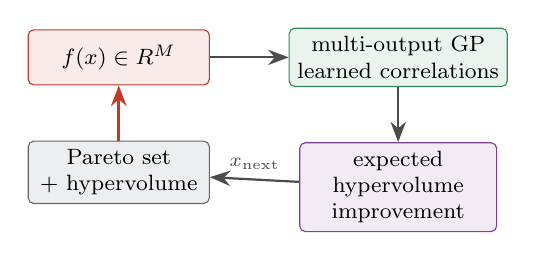
\begin{tikzpicture}[node distance=6mm and 8mm]
      \node[boxr, minimum width=2.3cm] (f) {$f(x)\in\mathbb{R}^M$};
      \node[boxg, minimum width=2.5cm, right=10mm of f] (gp) {multi-output GP\\ learned correlations};
      \node[boxp, minimum width=2.5cm, below=7mm of gp] (a) {expected\\ hypervolume\\ improvement};
      \node[boxk, minimum width=2.3cm, below=7mm of f] (p) {Pareto set\\ + hypervolume};
      \draw[flow] (f) -- (gp);
      \draw[flow] (gp) -- (a);
      \draw[flow] (a) -- node[above, lbl]{$x_{\rm next}$} (p);
      \draw[flowr] (p) -- (f);
    \end{tikzpicture}

    \smallskip\raggedright\footnotesize
    \begin{itemize}
      \item Per-objective min/max flags (\code{AcqConfig(maximize=[\dots])}).
      \item Reference point built from the initial data, then kept fixed so hypervolumes are comparable over iterations.
      \item Anti-correlated objectives can be learned automatically.
    \end{itemize}

    \column{0.44\textwidth}
    \centering
    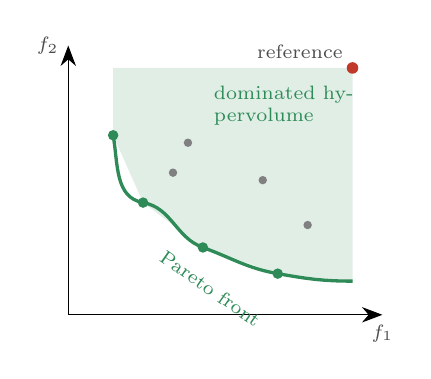
\begin{tikzpicture}[scale=0.95]
      \draw[->] (0,0) -- (4.2,0) node[below, lbl]{$f_1$};
      \draw[->] (0,0) -- (0,3.6) node[left, lbl]{$f_2$};
      % dominated region
      \fill[rambogreen!15] (0.6,3.3) -- (0.6,2.4) -- (1.0,1.5) -- (1.8,0.9) -- (2.8,0.55) -- (3.8,0.45) -- (3.8,3.3) -- cycle;
      \draw[rambogreen, very thick] (0.6,2.4) to[out=-80,in=170] (1.0,1.5) to[out=-10,in=160] (1.8,0.9) to[out=-20,in=170] (2.8,0.55) to[out=-10,in=180] (3.8,0.45);
      \foreach \x/\y in {0.6/2.4, 1.0/1.5, 1.8/0.9, 2.8/0.55}{ \fill[rambogreen] (\x,\y) circle (2pt); }
      \foreach \x/\y in {1.6/2.3, 2.6/1.8, 3.2/1.2, 1.4/1.9}{ \fill[black!50] (\x,\y) circle (1.6pt); }
      \fill[rambored] (3.8,3.3) circle (2.2pt) node[above left, lbl]{reference};
      \node[lbl, rambogreen, text width=2cm] at (3.0,2.8) {dominated hypervolume};
      \node[lbl, rambogreen, rotate=-35] at (1.9,0.35) {Pareto front};
    \end{tikzpicture}

    {\scriptsize Sketch: green = non-dominated points, grey = dominated. BO maximizes the shaded hypervolume.}
  \end{columns}
\end{frame}

% =============================================================== 14
\begin{frame}[fragile]{Feature: persistence and replay}
  \begin{columns}[T]
    \column{0.5\textwidth}
    Every run lands in its own folder (\code{create\_timestamp} or \code{run\_<n>}); a run never overwrites another.

    \medskip
    \centering
    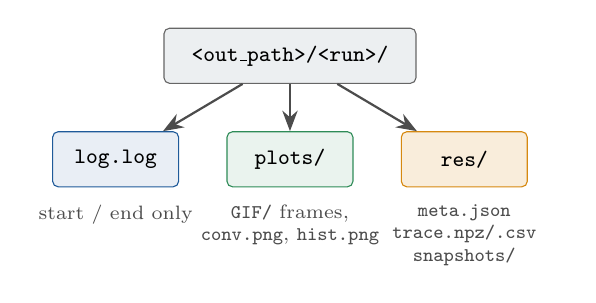
\begin{tikzpicture}[node distance=3.5mm and 6mm, font=\footnotesize]
      \node[boxk, minimum width=3.2cm] (run) {\code{<out\_path>/<run>/}};
      \node[box, below left=6mm and -2mm of run, minimum width=1.6cm] (log) {\code{log.log}};
      \node[boxg, below=6mm of run, minimum width=1.6cm] (plots) {\code{plots/}};
      \node[boxo, below right=6mm and -2mm of run, minimum width=1.6cm] (res) {\code{res/}};
      \draw[flow] (run) -- (log); \draw[flow] (run) -- (plots); \draw[flow] (run) -- (res);
      \node[lbl, below=1mm of plots, text width=2.3cm, align=center] (pl) {\code{GIF/} frames,\\ \code{conv.png}, \code{hist.png}};
      \node[lbl, below=1mm of log, text width=2.0cm, align=center] {start / end only};
      \node[lbl, below=1mm of res, text width=2.4cm, align=center] {\code{meta.json}\\ \code{trace.npz/.csv}\\ \code{snapshots/}};
    \end{tikzpicture}

    \column{0.48\textwidth}
    \textbf{Two tiers}
    \begin{itemize}\footnotesize
      \item \textbf{Tier 1 -- trace} (always): $x$, $y$, best, time, acquisition value, GP hyperparameters per iteration.
      \item \textbf{Tier 2 -- snapshots} (opt-in): what is needed to refit the GP \emph{exactly}; never dense covariance factors.
    \end{itemize}
\begin{lstlisting}
cfg = bo.SaveConfig(
    out_path="runs",
    snapshot_enabled=True)
res = bo.bayesian_optimization(
    ..., save_cfg=cfg)
run = bo.load_run(res.out_path)
run.posterior(7).predict(Xgrid)
\end{lstlisting}
    \footnotesize Reload months later, re-plot any iteration, no objective call. Plain \code{numpy}/JSON/CSV: no HDF5, no pickle.
  \end{columns}
\end{frame}

% =============================================================== 15
\begin{frame}{Feature: built-in visualization and logging}
  \begin{columns}[T]
    \column{0.5\textwidth}
    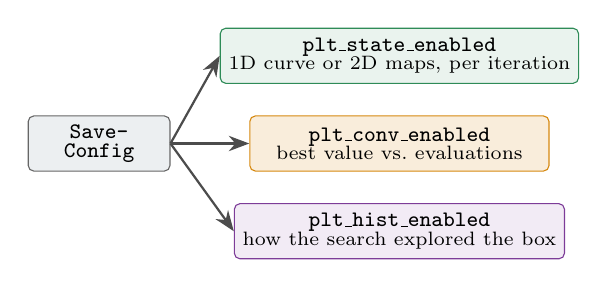
\begin{tikzpicture}
      \node[boxo, minimum width=3.8cm] (cv) {\code{plt\_conv\_enabled}\\[-1mm]\scriptsize best value vs.\ evaluations};
      \node[boxg, minimum width=3.8cm, above=4mm of cv] (st) {\code{plt\_state\_enabled}\\[-1mm]\scriptsize 1D curve or 2D maps, per iteration};
      \node[boxp, minimum width=3.8cm, below=4mm of cv] (hs) {\code{plt\_hist\_enabled}\\[-1mm]\scriptsize how the search explored the box};
      \node[boxk, minimum width=1.8cm, left=10mm of cv] (sc) {\code{Save-}\\[-1mm]\code{Config}};
      \draw[flow] (sc.east) -- (st.west);
      \draw[flow] (sc.east) -- (cv.west);
      \draw[flow] (sc.east) -- (hs.west);
    \end{tikzpicture}

    \column{0.46\textwidth}
    \begin{itemize}
      \item \code{plt\_all=True} is the master switch; \code{plot\_every=k} thins the frames; \code{dpi} is configurable.
      \item Frames are numbered \code{it\_XXX.png}, ready to assemble into a \textbf{GIF} of the optimization.
      \item The plotting module is imported \textbf{lazily}: headless / HPC runs do not need a matplotlib backend.
      \item The state plot marks what was evaluated this iteration and, with refinement, the ADAM endpoints.
    \end{itemize}
  \end{columns}
\end{frame}

% =============================================================== 16
\begin{frame}{Case study: feedback control of a Burgers wave (\code{advanced\_cases/})}
  \centering
  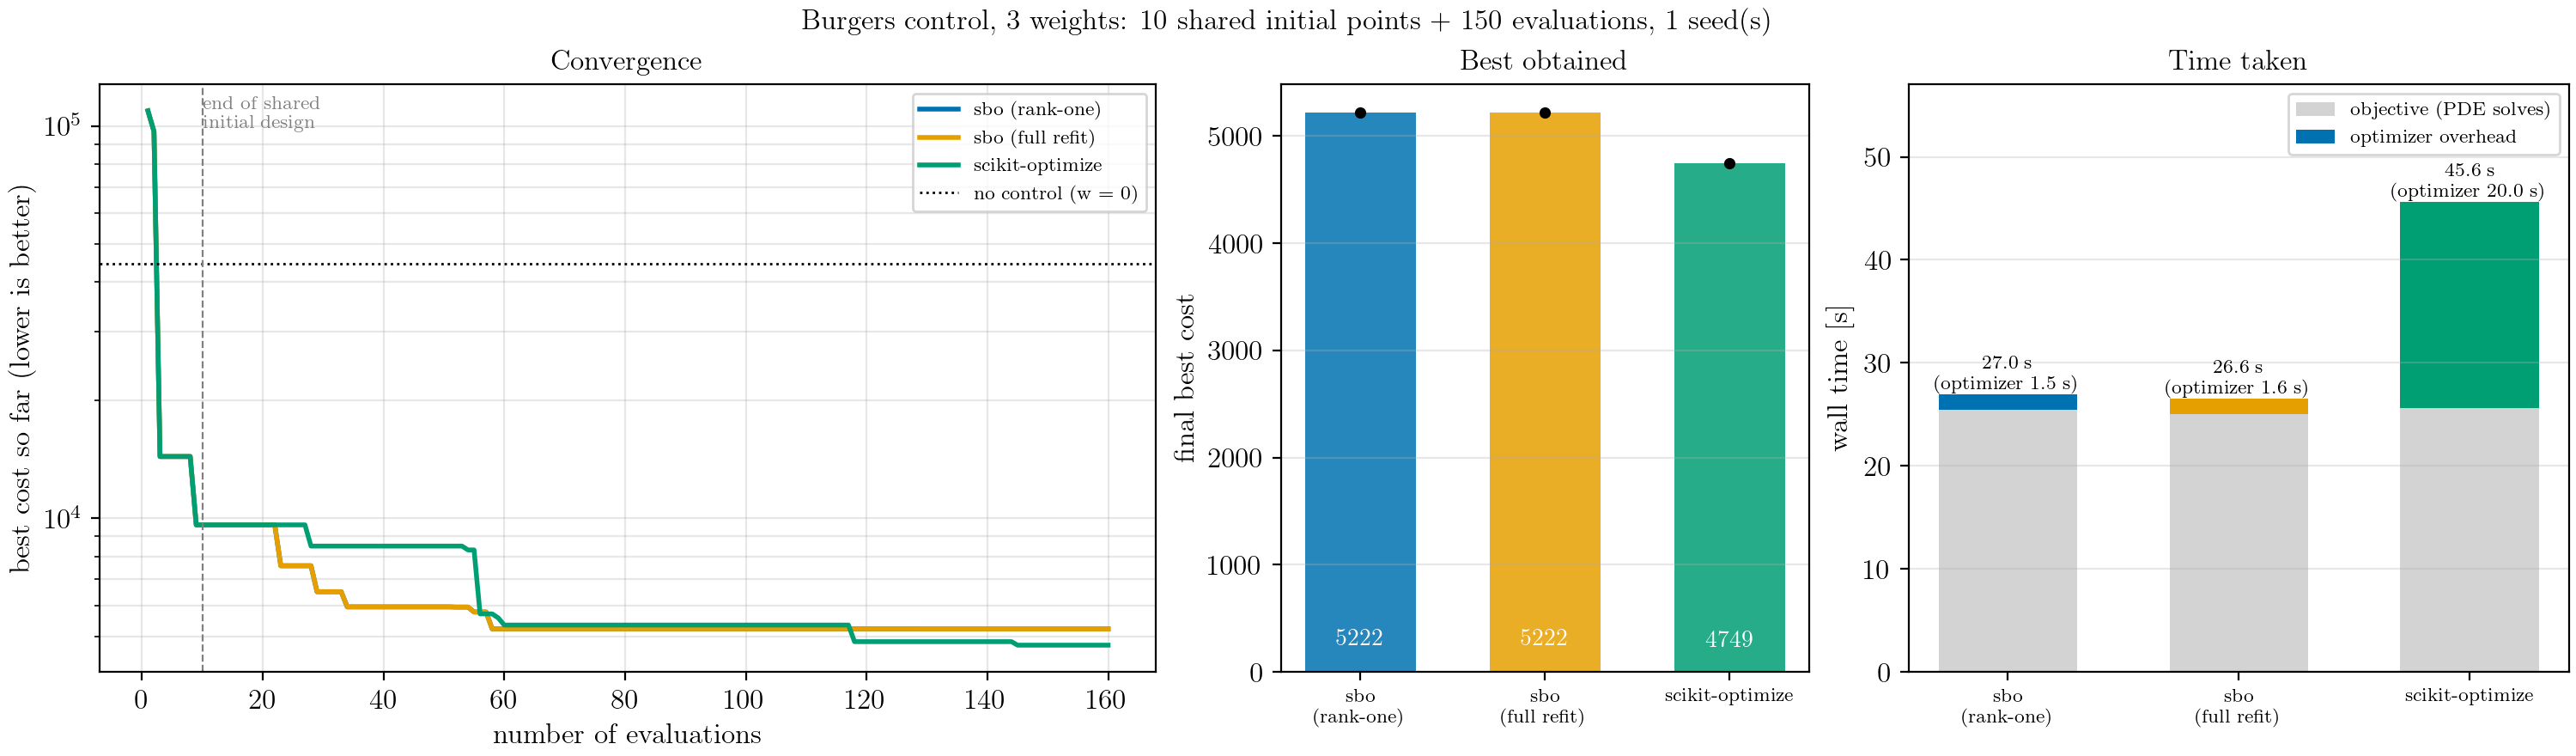
\includegraphics[width=0.86\textwidth]{figures/burgers_comparison.png}

  \smallskip
  \begin{columns}[T]
    \column{0.36\textwidth}
    \footnotesize
    \textbf{Task.} Tune 3 weights $w$ of a linear feedback law that damps a perturbed Burgers wave. One evaluation $=$ one PDE simulation (${\sim}0.2$\,s).

    \smallskip
    \centering
    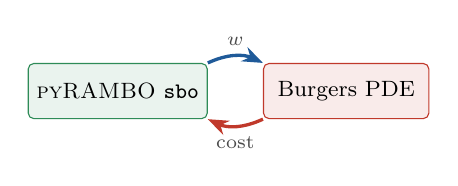
\begin{tikzpicture}[node distance=4mm and 7mm]
      \node[boxg, minimum width=2.1cm] (b) {\pr{} \code{sbo}};
      \node[boxr, minimum width=2.1cm, right=of b] (e) {Burgers PDE};
      \draw[flowb] (b.north east) to[bend left=25] node[above, lbl]{$w$} (e.north west);
      \draw[flowr] (e.south west) to[bend left=25] node[below, lbl]{cost} (b.south east);
    \end{tikzpicture}

    \column{0.62\textwidth}
    \footnotesize
    Same cost and same initial design for rank-one, full refit and \code{scikit-optimize} (1 seed, 150 evaluations):
    \begin{itemize}
      \item All three beat \textbf{no control} by a large factor.
      \item Optimizer overhead $\approx$1.5\,s for \code{sbo} vs.\ 20\,s for \code{skopt}.
      \item \code{skopt} reached a somewhat lower final cost here (4749 vs.\ 5222): one seed, not a ranking.
    \end{itemize}
  \end{columns}
\end{frame}

% =============================================================== 17
\begin{frame}{Quality, repository layout and where to start}
  \begin{columns}[T]
    \column{0.5\textwidth}
    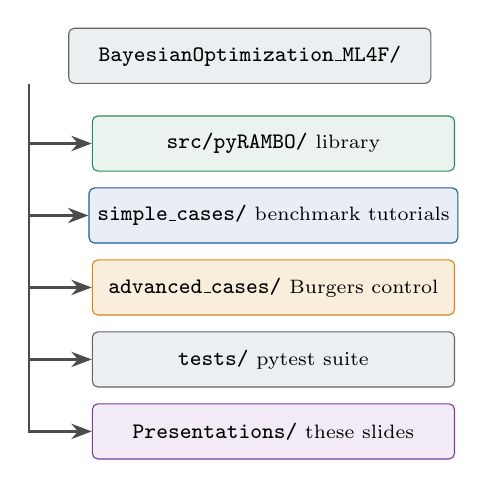
\begin{tikzpicture}[node distance=3mm]
      \node[boxk, minimum width=4.6cm, align=left] (r) {\code{BayesianOptimization\_ML4F/}};
      \node[boxg, minimum width=4.6cm, below=4mm of r, xshift=3mm] (a) {\code{src/pyRAMBO/}  \scriptsize library};
      \node[box, minimum width=4.6cm, below=2mm of a] (b) {\code{simple\_cases/}  \scriptsize benchmark tutorials};
      \node[boxo, minimum width=4.6cm, below=2mm of b] (c) {\code{advanced\_cases/}  \scriptsize Burgers control};
      \node[boxk, minimum width=4.6cm, below=2mm of c] (d) {\code{tests/}  \scriptsize pytest suite};
      \node[boxp, minimum width=4.6cm, below=2mm of d] (e) {\code{Presentations/}  \scriptsize these slides};
      \foreach \n in {a,b,c,d,e}{ \draw[flow] ([xshift=-5mm]r.south west |- r.south) |- (\n.west); }
    \end{tikzpicture}

    \column{0.48\textwidth}
    \textbf{Tutorials} cover: 1D and 2D benchmarks, large-scale normalization, persistence demo, Forrester multi-fidelity, Schaffer and Binh--Korn multi-objective.

    \medskip
    \textbf{Tests} include a numerical check that rank-one updates reproduce a full refit, plus refinement and persistence tests.

    \medskip
    \begin{block}{Try it}
      \footnotesize
      \code{pip install -e ".[test]"}\\
      \code{pytest}\\
      start from the 1D example in \code{simple\_cases/sbo/}
    \end{block}
  \end{columns}
\end{frame}

% =============================================================== 18
\begin{frame}{Summary and outlook}
  \begin{columns}[T]
    \column{0.52\textwidth}
    \begin{block}{Take-aways}
      \begin{itemize}\small
        \item One loop, \textbf{three flavours}: single-objective, multi-fidelity, multi-objective.
        \item Everything is a \textbf{dataclass config}; the driver is one function call.
        \item Speed features for expensive settings: rank-one updates, batches, gradient refinement.
        \item Runs are \textbf{reproducible}: folders, traces, snapshots, replay.
        \item Light dependencies, tested, with tutorials.
      \end{itemize}
    \end{block}
    \column{0.44\textwidth}
    \begin{exampleblock}{In progress (from the repo notes)}
      \small
      \begin{itemize}
        \item Port the new run layout, best-so-far semantics and refinement from \code{sbo} to \code{mfbo} and \code{mobo}.
        \item More than two fidelity levels (recursive formulation).
        \item JOSS paper submission.
      \end{itemize}
    \end{exampleblock}
    \centering\small
    \medskip
    \url{https://github.com/mendezVKI/BayesianOptimization_ML4F}\\[1mm]
    \textbf{Thank you -- questions?}
  \end{columns}
\end{frame}

\end{document}
